\section{Đề ôn thi giữa kỳ 2 toán 10}
\subsection{Phần trắc nghiệm}
Câu trắc nghiệm nhiều phương án lựa chọn. Học sinh trả lời từ
câu 1 đến câu 12. Mỗi câu hỏi học sinh \textit{chỉ chọn một} phương án.

\Opensolutionfile{ans}[Ans/Dapan]
 
\hienthiloigiaiex
%%%============EX_1==============%%%
\begin{ex}%[0D7N1-1]%[Dự án đề kiểm tra Toán khối 10 GHKII NH23-24-Dot 2 - Lê Hải Phụng]%[Deso 8 - CTST]
	Tìm khẳng định đúng trong các khẳng định sau:
	\choice
	{\True $f(x)=3x^2-5$ là tam thức bậc hai}
	{$f(x)=2x-4$ là tam thức bậc hai}
	{$f(x)=3x^3+2x-1$ là tam thức bậc hai}
	{$f(x)=x^4-x^2+1$ là tam thức bậc hai}
	\loigiai{$f(x)=3x^2-5$ là tam thức bậc hai.}
\end{ex}

\begin{ex}%[0D7V2-6]%[Dự án đề kiểm tra Toán khối 10 GHKII NH23-24-Dot 2 - Lê Hải Phụng]%[Deso 8 - CTST]
	Tập hợp các giá trị của tham số $m$ để bất phương trình $-x^2+2x-m-1>0$ vô nghiệm là 
	\choice
	{$(0;+\infty)$}
	{$(-\infty;0)$}
	{$(-\infty;0]$}
	{\True $[0;+\infty)$}
	\loigiai{Để bất phương trình $-x^2+2x-m-1>0$ vô nghiệm tức $-x^2+2x-m-1\le0$, $\forall x \in \mathbb{R}$.\\
		Tương đương ta có điều kiện $\heva{&-1<0\\&\Delta \le 0} \Rightarrow -4m \le 0 \Rightarrow m \ge 0$.}
\end{ex}
\begin{ex}%[0D7H2-1]%[Dự án đề kiểm tra Toán khối 10 GHKII NH23-24-Dot 2 - Lê Hải Phụng]%[Deso 8 - CTST]
	Tập nghiệm của bất phương trình $x^2+9>6x$ là
	\choice
	{\True $\mathbb{R}\setminus \{3\}$}
	{$\mathbb{R}$}
	{$(3;+\infty)$}
	{$(-\infty;3)$}
	\loigiai{Ta có $x^2+9>6x\Rightarrow x^2-6x+9>0$ $\Rightarrow (x-3)^2>0$, $\forall x \ne 3$.}
\end{ex}

\begin{ex}%[0D7H2-1]%[Dự án đề kiểm tra Toán khối 10 GHKII NH23-24-Dot 2 - Lê Hải Phụng]%[Deso 8 - CTST]
	Tập nghiệm $S$ của bất phương trình $\dfrac{-1}{x^2-3x-4}<0$ là
	\choice
	{$S=\mathbb{R}\setminus \{1;4\}$}
	{$S=[1;4]$}
	{\True $(-\infty;-1)\cup (4;+\infty)$}
	{$(-\infty;-1]\cup [4;+\infty)$}
	\loigiai{Ta có $\dfrac{-1}{x^2-3x-4}<0\Rightarrow x^2-3x-4>0 \Rightarrow x \in (-\infty;-1)\cup (4;+\infty)$.}
\end{ex}

\begin{ex}%[0D7H3-1]%[Dự án đề kiểm tra Toán khối 10 GHKII NH23-24-Dot 2 - Lê Hải Phụng]%[Deso 8 - CTST]
	Phương trình $\left(x^2-6x\right)\sqrt{17-x^2}=x^2-6x$ có bao nhiêu nghiệm thực phân biệt?
	\choice
	{$2$}
	{$1$}
	{$4$}
	{\True $3$}
	\loigiai{
		Điều kiện của phương trình là $17-x^2 \geq 0 \Leftrightarrow x^2 \leq 17$. Khi đó ta có
		$$\begin{aligned}
			&\left(x^2-6x\right)\sqrt{17-x^2}=x^2-6x 
			\Leftrightarrow \left(x^2-6x\right)\left(\sqrt{17-x^2}-1\right)=0 \\
			\Leftrightarrow~ 
			&\hoac{&x^2-6x=0\\&\sqrt{17-x^2}=1}
			\Leftrightarrow \hoac{&x=0 \text{ hoặc } x=6\\&17-x^2=1}
			\Leftrightarrow \hoac{&x=0 \text{ hoặc } x=6\\&x=-4 \text{ hoặc } x=4.}
		\end{aligned}$$
		Ba số $x=0$, $x=\pm 4$ thỏa mãn điều kiện $x^2 \leq 17$ và thỏa mãn phương trình.\\
		Vậy phương trình đã cho có $3$ nghiệm là $x=0$ và $x=\pm 4$.
	}
\end{ex}

\begin{ex}%[0D7N3-2]%[Dự án đề kiểm tra Toán khối 10 GHKII NH23-24-Dot 2 - Lê Hải Phụng]%[Deso 8 - CTST]
	Điều kiện xác định của phương trình $\sqrt{2x-1}=4x+1$ là
	\choice
	{$(1;+\infty)$}
	{\True $\left[\dfrac{1}{2};+\infty \right) $}
	{$\left[-\dfrac{1}{2};+\infty \right) $}
	{$\left( -\infty;\dfrac{1}{2}\right] $}
	\loigiai{Điều kiện xác định: $2x+1\ge 0\Rightarrow x\ge \dfrac{1}{2}$.}
\end{ex}


\begin{ex}%[0H9N2-5]%[Dự án đề kiểm tra Toán khối 10 GHKII NH23-24-Dot 2 - Lê Hải Phụng]%[Deso 8 - CTST]
	Trong mặt phẳng tọa độ $Oxy$, cho hai điểm $A(-4;5)$ và $B(8;-1)$. Điểm $P$ thuộc trục hoành sao cho $A$, $B$, $P$ thẳng hàng. Tọa độ $P$ là
	\choice
	{$(0;3)$}
	{$(0;-3)$}
	{$(-6;0)$}
	{\True $(6;0)$}
	\loigiai{Do $P \in Ox$ nên $P(x;0)$. Ta có $\overrightarrow{AB}=(12;-6)$ và $\overrightarrow{AP}=(x+4;-5)$. Vì $A$, $P$, $B$ thẳng hàng nên $\dfrac{x+4}{12}=\dfrac{-5}{-6}$. Vậy $P(6;0)$.}
\end{ex}

\begin{ex}%[0H9N2-5]%[Dự án đề kiểm tra Toán khối 10 GHKII NH23-24-Dot 2 - Lê Hải Phụng]%[Deso 8 - CTST]
	Trong mặt phẳng tọa độ, cho hai điểm $A(1;5)$ và $B(3;2)$. Điểm $C$ đối xứng với $A$ qua $B$ có tọa độ là
	\choice
	{\True $(5;-1)$}
	{$\left(2;\dfrac{7}{2} \right)  $}
	{$(-1;8)$}
	{$(5;1)$}
	\loigiai{Giả sửa $C(a;b)$. Ta có $\heva{&\dfrac{a+1}{2}=3\\&\dfrac{b+5}{2}=2}\Rightarrow \heva{&a=5\\&b=-1}$. Vậy $C(5;-1)$.}
\end{ex}

\begin{ex}%[0H9N2-5]%[Dự án đề kiểm tra Toán khối 10 GHKII NH23-24-Dot 2 - Lê Hải Phụng]%[Deso 8 - CTST]
	Đường thẳng $51x-30y+11=0$ đi qua điểm nào sau đây?
	\choice
	{$\left(-1;\dfrac{3}{4} \right) $}
	{\True $\left(-1;-\dfrac{4}{3} \right) $}
	{$\left(1;\dfrac{3}{4} \right) $}
	{$\left(-1;-\dfrac{3}{4} \right) $}
	\loigiai{Ta có tọa độ $\left(-1;-\dfrac{4}{3} \right) $ thì phương trình đường thẳng thỏa mãn.}
\end{ex}

\begin{ex}%[0H9N3-5]%[Dự án đề kiểm tra Toán khối 10 GHKII NH23-24-Dot 2 - Lê Hải Phụng]%[Deso 8 - CTST]
	Khoảng cách từ điểm $M(1;-1)$ đến đường thẳng $\Delta : -3x+4y-3=0$ bằng
	\choice
	{$\dfrac{4}{5}$}
	{\True $2$}
	{$\dfrac{4}{\sqrt{5}}$}
	{$\dfrac{10}{\sqrt{5}}$}
	\loigiai{$d(M;\Delta)=\dfrac{|-3\cdot 1+4\cdot(-1)-3|}{\sqrt{3^2+4^2}}=2$.}
\end{ex}

\begin{ex}%%[0H9H4-2]%[Dự án đề kiểm tra Toán khối 10 GHKII NH23-24-Dot 2 - Lê Hải Phụng]%[Deso 8 - CTST]
	Trong mặt phẳng tọa độ, cho hai điểm $A(1;1)$ và $B(7;5)$. Phương trình của đường tròn đường kính $AB$ là
	\choice
	{$x^2+y^2+8x+6y+12=0$}
	{\True $x^2+y^2-8x-6y+12=0$}
	{$x^2+y^2-8x-6y-12=0$}
	{$x^2+y^2+8x+6y-12=0$}
	\loigiai{Ta có tâm $I$ của đường tròn là trung điểm của $AB$ suy ra $I(4;3)$.\\
		Bán kính của đường tròn $R=\dfrac{AB}{2}=\sqrt{13}$.\\
		Suy ra phương trình đường tròn đường kính $AB$ có dạng $(x-4)^2+(y-3)^2=13$ hay $x^2+y^2-8x-6y+12=0$.}
\end{ex}

\begin{ex}%[0H9H4-3]%[Dự án đề kiểm tra Toán khối 10 GHKII NH23-24-Dot 2 - Lê Hải Phụng]%[Deso 8 - CTST]
	Phương trình tiếp tuyến của đường tròn $x^2+y^2-2x-4y-3=0$ tại điểm $M(3;4)$ là
	\choice
	{\True $x+y-7=0$}
	{$x+y+7=0$}
	{$x-y-7=0$}
	{$x+y-3=0$}
	\loigiai{Phương trình đường tròn $x^2+y^2-2x-4y-3=0$ có tâm $I(1;2)$.\\
		Tiếp tuyến của đường tròn qua $M(3;4)$ và có VTPT là $\overrightarrow{IM}=(2;2)$ nên tiếp tuyến có phương trình tổng quát $x+y-7=0$.}
\end{ex}
  
\Closesolutionfile{ans}
\bangdapan{Dapan}

\subsection{Câu trắc nghiệm đúng sai}
Học sinh trả lời từ câu 1 đến câu 4.
Trong mỗi ý \circlenum{A}, \circlenum{B}, \circlenum{C} và \circlenum{D} ở mỗi câu, học sinh chọn đúng hoặc sai.
\setcounter{ex}{0}
\LGexTF
\Opensolutionfile{ansbook}[ansbook/DapanDS]
\Opensolutionfile{ans}[Ans/DapanT]
%%%============EX_1==============%%%
\begin{ex}%[0D7V1-2]%[Dự án đề kiểm tra Toán khối 10 GHKII NH23-24-Dot 2 - An Do]%[Deso 8 - CTST]
	Xét tính đúng, sai của các khẳng định sau:
	\choiceTF
	{$f(x)=2x^2-5x+2$ có $f(x) > 0, \forall x \in\left(\dfrac{1}{2}; 2\right)$}
	{\True $f(x)=9-x^2$ có $f(x) > 0, \forall x \in(-3; 3)$}
	{\True $f(x)=x^2-(\sqrt{7}-1) x+\sqrt{3}$ có $f(x) > 0, \forall x \in \mathbb{R}$}
	{\True $f(x)=-x^2+x-\dfrac{1}{4}$ có $f(x) < 0, \forall x \in \mathbb{R} \setminus\left\{\dfrac{1}{2}\right\}$}
	\loigiai{
		\begin{enumerate}
			\item $f(x) = 2x^2 - 5x + 2$ ($a = 2, b = -5, c =2$).
			\\Ta có $\Delta = (-5)^2 - 4\cdot 2\cdot 2 = 9 >0$; $f(x)$ có hai nghiệm phân biệt $x_1=2, x_2 = \dfrac{1}{2}$.
			\\Bảng xét dấu $f(x)$:
			\begin{center}
				\begin{tikzpicture}
					\foreach \x [count=\i from 0] in {-\infty,\dfrac{1}{2},2,+\infty} %i đang 0 đến 4
					{\path (2*\i,0) node {$\x$};\global\let\n=\i} %Gán giá trị n=i, đang là 4
					\foreach \y [count=\i from 0] in {x,f(x)} %i đang 0 đến 2
					{\draw	(-3,-\i-0.5)--(2*\n+0.5,-\i-0.5) %Kẻ hàng ngang
						(-1.75,-\i) node {$\y$};\global\let\m=\i}	%Gán giá trị m=i, đang là 2
					\foreach \x [count=\i from 1] in {+,0,-,0,+}
					{\path	 (\i,-1) node {$\x$};}
					\draw 	(-3,0.5) rectangle (2*\n+0.5,-\m-0.5) %Vẽ viền xung quanh
					(-0.5,0.5)--(-0.5,-\m-0.5);%Vẽ đường gạch xuống
				\end{tikzpicture}
			\end{center}
			Kết luận $f(x)>0, \forall x \in\left(-\infty ; \dfrac{1}{2}\right) \cup(2 ;+\infty) ; f(x)<0, \forall x \in\left(\dfrac{1}{2} ; 2\right)$.
			\item $f(x)=9-x^2 ;(a=-1, b=0, c=9)$.\\
			Ta có: $\Delta=0^2-4 \cdot(-1) \cdot 9=36>0 ; f(x)$ có hai nghiệm phân biệt là $x_1=-3, x_2=3$.
			\\Bảng xét dấu $f(x)$
			\begin{center}
				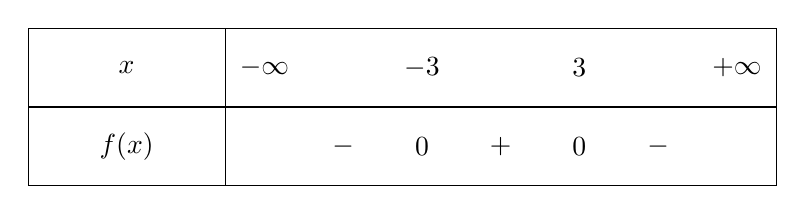
\begin{tikzpicture}
					\foreach \x [count=\i from 0] in {-\infty,-3,3,+\infty} %i đang 0 đến 4
					{\path (2*\i,0) node {$\x$};\global\let\n=\i} %Gán giá trị n=i, đang là 4
					\foreach \y [count=\i from 0] in {x,f(x)} %i đang 0 đến 2
					{\draw	(-3,-\i-0.5)--(2*\n+0.5,-\i-0.5) %Kẻ hàng ngang
						(-1.75,-\i) node {$\y$};\global\let\m=\i}	%Gán giá trị m=i, đang là 2
					\foreach \x [count=\i from 1] in {-,0,+,0,-}
					{\path	 (\i,-1) node {$\x$};}
					\draw 	(-3,0.5) rectangle (2*\n+0.5,-\m-0.5) %Vẽ viền xung quanh
					(-0.5,0.5)--(-0.5,-\m-0.5);%Vẽ đường gạch xuống
				\end{tikzpicture}
			\end{center}
			Kết luận $f(x) > 0, \forall x \in (-3;3); f(x) < 0, \forall x \in (-\infty;-3)\cup (3; +\infty)$.
			\item $f(x)=x^2-(\sqrt{7}-1) x+\sqrt{3}$ ($a = 1, b = -\sqrt{7}, c = \sqrt{3}$).
			\\Ta có $\Delta = \left[-\left(1-\sqrt{7}\right)\right]^2 - 4\cdot 1\cdot \sqrt{3} = 8-2\sqrt{7} - 4\sqrt{3} <0$.
			\\Bảng xét dấu $f(x)$
			\begin{center}
				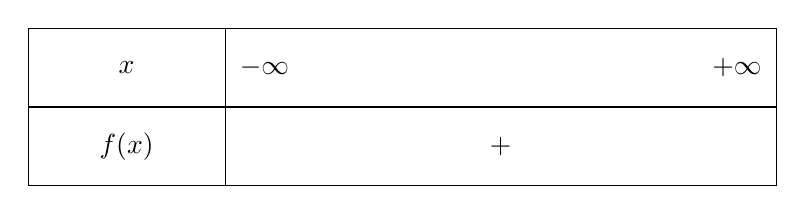
\begin{tikzpicture}
					\foreach \x [count=\i from 0] in {-\infty, , ,+\infty} %i đang 0 đến 4
					{\path (2*\i,0) node {$\x$};\global\let\n=\i} %Gán giá trị n=i, đang là 4
					\foreach \y [count=\i from 0] in {x,f(x)} %i đang 0 đến 2
					{\draw	(-3,-\i-0.5)--(2*\n+0.5,-\i-0.5) %Kẻ hàng ngang
						(-1.75,-\i) node {$\y$};\global\let\m=\i}	%Gán giá trị m=i, đang là 2
					\foreach \x [count=\i from 1] in { , ,+, , }
					{\path	 (\i,-1) node {$\x$};}
					\draw 	(-3,0.5) rectangle (2*\n+0.5,-\m-0.5) %Vẽ viền xung quanh
					(-0.5,0.5)--(-0.5,-\m-0.5);%Vẽ đường gạch xuống
				\end{tikzpicture}
			\end{center}
			Kết luận $f(x) > 0, \forall x \in \mathbb{R}$.
			\item $f(x)=-x^2+x-\dfrac{1}{4} ;\left(a=-1, b=1, c=-\dfrac{1}{4}\right)$.\\
			Ta có: $\Delta=1^2-4(-1) \cdot\left(-\dfrac{1}{4}\right)=0 ; f(x)$ có nghiệm kép $x=\dfrac{1}{2}$.\\
			Bảng xét dấu $f(x)$
			\begin{center}
				\begin{tikzpicture}
					\foreach \x [count=\i from 0] in {-\infty, ,\dfrac{1}{2}, ,+\infty} %i đang 0 đến 4
					{\path (2*\i,0) node {$\x$};\global\let\n=\i} %Gán giá trị n=i, đang là 4
					\foreach \y [count=\i from 0] in {x,f(x)} %i đang 0 đến 2
					{\draw	(-3,-\i-0.5)--(2*\n+0.5,-\i-0.5) %Kẻ hàng ngang
						(-1.75,-\i) node {$\y$};\global\let\m=\i}	%Gán giá trị m=i, đang là 2
					\foreach \x [count=\i from 1] in { , -,,0, ,- ,}
					{\path	 (\i,-1) node {$\x$};}
					\draw 	(-3,0.5) rectangle (2*\n+0.5,-\m-0.5) %Vẽ viền xung quanh
					(-0.5,0.5)--(-0.5,-\m-0.5);%Vẽ đường gạch xuống
				\end{tikzpicture}
			\end{center}
			Kết luận $f(x) < 0, \forall x \in \mathbb{R}\setminus\left\{\dfrac{1}{2}\right\}$.
		\end{enumerate}
	}
\end{ex}

\begin{ex}%[0D7V3-1]%[Dự án đề kiểm tra Toán khối 10 GHKII NH23-24-Dot 2 - An Do]%[Deso 8 - CTST]
	Cho phương trình $(x+1)\left(\sqrt{x+4}-\sqrt{-x^2 + 4x + 14} = 0\right)$ ($*$). Khi đó
	\choiceTF{Điều kiện $x \geq 4$}
	{\True Phương trình (*) có $3$ nghiệm phân biệt}
	{Các nghiệm của phương trình (*) nhỏ hơn $5$}
	{\True Tổng các nghiệm của phương trình $(*)$ bằng $2$}
	\loigiai{
		Ta có $(x+1)\left(\sqrt{x+4}-\sqrt{-x^2+4 x+14}\right)=0 \Leftrightarrow\hoac{&x+1=0 \\
			&\sqrt{x+4}-\sqrt{-x^2+4 x+14}=0.}$\\
		Phương trình $x+1=0$ có nghiệm là $x=-1$.\\
		Ta có: $\sqrt{x+4}-\sqrt{-x^2+4 x+14}=0 \Leftrightarrow \sqrt{x+4}=\sqrt{-x^2+4 x+14}$ ($1$)\\
		Bình phương hai vế phương trình ($1$) ta có\\ $x+4=-x^2+4 x+14 \Leftrightarrow x^2-3 x-10=0 \Leftrightarrow x=5$ hoặc $x=-2$ (đều thoả mãn $x+4 \geq 0$ ). 
		\\Vậy tập nghiệm của phương trình ban đầu là $S=\{-2 ;-1 ; 5\}$.
	}
\end{ex}

\begin{ex}%[Dự án đề kiểm tra Toán khối 10 GHKII NH23-24-Dot 2 - An Do]%[Deso 8 - CTST]
	Cho tam giác $ABC$ có phương trình đường thẳng $BC$ là $7x + 5y - 8 = 0$, phương trình các đường cao kẻ từ $B, C$ lần lượt là $9x - 3y - 4 = 0, x + y - 2 =0$. Lập phương trình đường cao và đường trung tuyến kẻ từ $A$. Khi đó:
	\choiceTF
	{\True Điểm $B$ có tọa độ là  $\left(\dfrac{2}{3}; \dfrac{2}{3}\right)$}
	{\True Điểm $C$ có tọa độ là $(1; -3)$}
	{Phương trình đường cao kẻ từ $A$ là $5x - 7y -6 = 0$}
	{Phương trình đường trung tuyến kẻ từ $A$ là $x - 13y + 4 = 0$}
	\loigiai{
		Toạ độ của điểm $B$ là nghiệm của hệ phương trình\\ $\heva{&7 x+5 y-8=0 \\
			&9 x-3 y-4=0} \Leftrightarrow\heva{&x=\dfrac{2}{3} \\
			&y=\dfrac{2}{3}.}$\\
		Suy ra điểm $B$ có toạ độ là $\left(\dfrac{2}{3} ; \dfrac{2}{3}\right)$.\\
		Toạ độ của điểm $C$ là nghiệm của hệ phương trình\\ $\heva{&7 x+5 y-8=0 \\
			&x+y-2=0} \Leftrightarrow\heva{&x=-1 \\
			&y=3.}$\\
		Suy ra điểm $C$ có tọa độ là $(-1 ; 3)$.\\
		Đường thẳng $AB$ đi qua điểm $B\left(\dfrac{2}{3} ; \dfrac{2}{3}\right)$ và nhận vectơ chỉ phương $\overrightarrow{u_1}=(1 ;-1)$ của đường cao kẻ từ $C$ làm vectơ pháp tuyến có phương trình là $(x+1)+3(y-3)=0 \Leftrightarrow x+3 y-8=0$.\\
		Toạ độ của điểm $A$ là nghiệm của hệ phương trình $\heva{&x-y=0 \\
			&x+3 y-8=0}\Leftrightarrow\heva{&x=2 \\
			&y=2.}$\\
		Suy ra điểm $A$ có toạ độ là $(2 ; 2)$.
		\\Phương trình đường cao kẻ từ $A(2; 2)$ và nhận vectơ chỉ phương $\overrightarrow{u}=(5;-7)$ của đường thẳng $BC$ làm vectơ pháp tuyến là $5(x-2) - 7(y-2) = 0 \Leftrightarrow 5x - 7y + 4 =0$.
		\\Gọi $I$ là trung điểm của $BC$, ta có tọa độ điểm $I$ là  $\left(\dfrac{-1}{6}; \dfrac{11}{6}\right)$.
		\\Do đó $\overrightarrow{IA} = \left(\dfrac{13}{6}; \dfrac{1}{6}\right)$.
		\\Đường trung tuyến kẻ từ $A$ nhận $\overrightarrow{n} = (1;-1)$ làm vectơ pháp tuyến, có phương trình là
		\\$(x-2) - 13(y-2) = 0 \Leftrightarrow x - 13y + 24 = 0$.
	}
\end{ex}

%%%============EX_1==============%%%
\begin{ex}%[0H9V3-7]%[Dự án đề kiểm tra Toán khối 10 GHKII NH23-24-Dot 2 - An Do]%[Deso 8 - CTST]
	Xác định tính đúng, sai của các khẳng định sau:
	\choiceTF
	{Phương trình $(C)$ có tâm $I(-1;-7)$ và bán kính $R=3\sqrt{3}$ là: $(x+1)^2+(y+7)^2=27$}
	{Phương trình $(C)$ có tâm $I(1;-5)$ và đi qua $O(0; 0)$ là: $(x-1)^2+(y+5)^2=26$}
	{Phương trình $(C)$ nhận $AB$ làm đường kính với $A(1; 1), B(7; 5)$ là: $(x-4)^2+(y-3)^2=10$}
	{Phương trình $(C)$ đi qua ba điểm: $M(-2; 4), N(5; 5), P(6;-2)$ là: $x^2+y^2-6x-2y-20=0$}
	\loigiai{
		\begin{enumerate}
			\item  Phương trình $(C):(x+1)^2+(y+7)^2=27$.
			\item  $(C)$ có bán kính $R=O I=\sqrt{(1-0)^2+(-5-0)^2}=\sqrt{26}$ nên có phương trình\\ $(x-1)^2+(y+5)^2=26$.
			\item  Gọi $I$ là trung điểm của đoạn $AB \Rightarrow I(4; 3) ; AI=\sqrt{(4-1)^2+(3-1)^2}=\sqrt{13}$. Đường tròn $(C)$ có đường kính là $AB$ suy ra $(C)$ nhận $I(4 ; 3)$ làm tâm và bán kính $R=AI=\sqrt{13}$ nên có phương trình là $(x-4)^2+(y-3)^2=13$.
			\item  Gọi phương trình đường tròn $(C)$ là: $x^2 + y^2 - 2ax- 2by + c=0$.\\
			Do đường tròn đi qua ba điểm $M, N, P$ nên ta có hệ phương trình:
			$$\heva{&4 + 16 + 4a - 8b + c=0\\
				&25 + 25 - 10a - 10b + c=0\\
				&36 + 4 - 12a + 4b + c=0}
			\Leftrightarrow \heva{&a =2 \\ &b = 1\\ &c =-20.}
			$$
			Vậy phương trình đường tròn $(C): x^2+y^2-4 x-2 y-20=0$.
		\end{enumerate}
		
	}
\end{ex}

\Closesolutionfile{ans}
\Closesolutionfile{ansbook}

\begin{center}
	\textbf{\textsf{BẢNG ĐÁP ÁN ĐÚNG SAI}}
\end{center}
\input{Ansbook/DapanDS}

\subsection{Phần tự luận}

\hienthiloigiaibt
%%%==============BT_1==============%%%
\begin{bt}%[0D7H1-2]
	Tìm tất cả các giá trị của tham số $m$ để phương trình $x^2-mx+m+3=0$ có nghiệm.
	\loigiai{
		Để phương trình $x^2-mx+m+3=0$ có nghiệm thì 
		\begin{eqnarray*}
			\Delta \ge 0\Leftrightarrow m^2-4\left(m+3\right)\ge 0\Leftrightarrow m^2-4m-12\ge 0\Leftrightarrow \hoac{&{m\le-2} \\
				&{m\ge 6.}}
		\end{eqnarray*}
	Vậy $m\leq -2$ hoặc $m\geq 6$ thì phương trình đã cho có nghiệm.
	}
\end{bt}

%%%==============BT_2==============%%%
\begin{bt}%[0D7V1-2]
	Tìm tập hợp tất cả các giá trị của tham số $m$ để hàm số $y=\sqrt{\left(m-10\right)x^2-2\left(m-10\right)x+1}$ có tập xác định là $\mathbb{R}$.
	\loigiai{
		Để hàm số đã cho có tập xác định là $\mathbb{R}$ thì
		\begin{eqnarray*}
			\left(m-10\right)x^2-2\left(m-10\right)x+1\ge 0,\forall x\in \mathbb{R}\quad(*).
		\end{eqnarray*}
	\begin{itemize}
		\item Với $m=10$ thì $(*)$ luôn đúng $\forall x\in \mathbb{R}$. Vậy $m=10$ thỏa mãn.
		\item Với $m\ne 10$ thì 
		\begin{eqnarray*}
			(*) &\Leftrightarrow& \heva{&{m-10> 0}\\&{\left(m-10\right)^2-\left(m-10\right)\le 0}&}
			 \Leftrightarrow \heva{&{m > 10} \\&{\left(m-10\right)\left(m-11\right)\le 0}&}\\
			 &\Leftrightarrow& \heva{&{m > 10} \\
				&{10\le m\le 11}&} \Rightarrow 10< m\le 11.
		\end{eqnarray*}
	\end{itemize}		
		Vậy $10\le m\le 11$ thì hàm số đã cho có tập xác định là $\mathbb{R}$.
	}
\end{bt}

%%%==============BT_3==============%%%
\begin{bt}%[0D7C3-2]
	Tập hợp tất cả các giá trị của tham số $m$ để phương trình $\sqrt{2x^2-6x+m}=x-1$ có $2$ nghiệm phân biệt là khoảng $\left[a;b\right)$ với $a,b\in \mathbb{N}^*$. Tính diện tích một tam giác vuông có cạnh huyền bằng $b$ và một cạnh góc vuông bằng $a$.
	\loigiai{
		\begin{eqnarray*}
			& &\sqrt{2x^2-6x+m}=x-1\Leftrightarrow \heva{&{x-1\ge 0} \\&{2x^2-6x+m=\left(x-1\right)^2}&}\\
			&\Leftrightarrow& \heva{&{x\ge 1} \\&{x^2-4x+m-1=0}&} \Leftrightarrow \heva{&{x\ge 1} \\&{m=-x^2+4x+1}}
		\end{eqnarray*}
		Xét hàm số $f(x)=-x^2+4x+1$ trên nửa khoảng $\left[1;+\infty \right)$.\\
		Ta có hàm số $f(x)=-x^2+4x+1$ có đồ thị làm một parabol đỉnh $I\left(2;5\right)$ và $a < 0$ nên ta có bảng biến thiên
		\begin{center}
			
\begin{tikzpicture}[>=stealth]
				\tkzTabInit[nocadre=false,lgt=1.2,espcl=2,deltacl=0.6]{$x$/.6 ,$f(x)$/2}
				{$1$ , $2$ , $+\infty$}
				\tkzTabVar{-/$4$ , +/$5$ , -/$-\infty$}
			\end{tikzpicture}
		\end{center}
		Dựa vào bảng biến thiên, ta thấy phương trình đã cho có hai nghiệm phân biệt khi và chỉ khi $m\in \left[4;5\right)$. Suy ra $a=4$, $b=5$.\\
		Khi đó, diện tích một tam giác vuông có cạnh huyền bằng $b$ và một cạnh góc vuông bằng $a$ là \[S=\dfrac{1}{2} a\sqrt{b^2-a^2}=6.\]
	}
\end{bt}

%%%==============BT_4==============%%%
\begin{bt}%[0H9H2-4]
	Cho tam giác $ABC$ có các đỉnh $A\left(1;1\right)$, $B\left(2;4\right)$, $C\left(10;-2\right)$. Tính diện tích tam giác $ABC$.
	\loigiai{
		Ta có $\overrightarrow{AB}=\left(1;3\right),\overrightarrow{AC}=\left(9;-3\right)$.\\
		Vì $\overrightarrow{AB}\cdot \overrightarrow{AC}=1\cdot 9+3\cdot \left(-3\right)=0$ nên $AB\perp AC$. Suy ra $\triangle ABC$ vuông tại $A$.\\
		Khi đó diện tích tam giác $ABC$ là $S=\dfrac{1}{2} AB\cdot AC=\dfrac{1}{2} \sqrt{1^2+3^2} \cdot \sqrt{9^2+\left(-3\right)^2}=15$.
	}
\end{bt}

%%%==============BT_5==============%%%
\begin{bt}%[0H9C3-5]
	Viết phương trình đường thẳng $\Delta$ đi qua điểm $M$ và cách đều các điểm $P$, $Q$ với $M\left(2;5\right)$, $P\left(-1;2\right)$, $Q\left(5;4\right)$.
	\loigiai{
		Vì đường thẳng $\Delta$ cách đều các điểm $P$, $Q$ nên $\Delta$ song song với đường thẳng $PQ$ hoặc $\Delta$ đi qua trung điểm của đoạn thẳng $PQ$.
		\begin{itemize}
			\item $\Delta$ song song với đường thẳng $PQ$ nên đường thẳng $\Delta$ nhận $\overrightarrow{PQ}=\left(6;2\right)$ làm véc-tơ chỉ phương.\\
			Khi đó phương trình tổng quát của đường thẳng $\Delta$ đi qua điểm $M\left(2;5\right)$ và nhận $\vec{n}=\left(1;-3\right)$ làm véc-tơ pháp tuyến là $x-3y+13=0$.
			\item $\Delta$ đi qua trung điểm $N\left(2;3\right)$ của đoạn thẳng $PQ$. Do đó $\Delta$ nhận $\overrightarrow{MN}=\left(0;-2\right)$ làm véc-tơ chỉ phương.\\
			Khi đó phương trình tổng quát của đường thẳng $\Delta$ đi qua điểm $M\left(2;5\right)$ và nhận $\vec{n}=\left(1;0\right)$ làm véc-tơ pháp tuyến là $x-2=0$.
		\end{itemize}
	Vậy có hai đường thẳng $\Delta$ thỏa mãn yêu cầu bài toán là $\Delta_1:x-3y+13=0$ và $\Delta_2:x-2=0$.
	}
\end{bt}

%%%==============BT_6==============%%%
\begin{bt}%[0H9C4-3]
	Cho số thực $\alpha$ $\left(0< \alpha < \dfrac{\pi}{4} \right)$. Góc giữa hai tiếp tuyến được vẽ từ điểm $P$ đến đường tròn có phương trình $x^2+y^2+6x+10y-3\sin^3 \alpha-4\cos \alpha \sin^2 \alpha+34=0$ là $2\alpha$. Quỹ tích điểm $P$ là hình tròn có bán kính bằng bao nhiêu?
	\loigiai{
		\begin{center}
			\begin{tikzpicture}
				\def\r{2}
				\path 	(0:0) coordinate (I) 
				(180:2*\r) coordinate (P)
				($(I)!.5!(P)$) coordinate (O);
				\path[name path=ciri](I) circle (\r);
				\path[name path=ciro](O) let\p1=($(O)-(I)$) in circle ({veclen(\x1,\y1)});
				\path[name intersections={of=ciri and ciro,by={A,B}}];
				\draw	(I) circle (\r) (A)--(P)--(B) (P)--(I)--(A) (I)--(B);
				\foreach \x/\g in {I/0,P/180,A/135,B/-135}
				\fill[black] 	(\x) circle (1pt)
				($(\g:3mm)+(\x)$) node {$\x$};
				\draw pic[draw,angle radius=3mm]{right angle=P--A--I}
					  pic[draw,angle radius=3mm]{right angle=P--B--I}
					  pic[draw,angle radius=4mm]{angle=B--P--I}
					  pic[draw,angle radius=5mm]{angle=I--P--A}
					   pic[draw=none,"$\alpha$",angle radius=12mm]{angle=I--P--A};
\end{tikzpicture}
		\end{center}
		Đường tròn $\left(C\right)$ đã cho có tâm $I\left(-3;-5\right)$, bán kính $R=\sqrt{3\sin^3 \alpha+4\cos \alpha \sin^2 \alpha}$.\\
		Gọi $P\left(x;y\right)$, xét tam giác $IAP$ ta có 
		\begin{eqnarray*}
			& & \sin \alpha=\dfrac{IA}{IP}=\dfrac{R}{IP}=\dfrac{\sqrt{3\sin^3 \alpha+4\cos \alpha \sin^2 \alpha}}{\sqrt{\left(x+3\right)^2+\left(y+5\right)^2}}\\
			&\Leftrightarrow& \left(x+3\right)^2+\left(y+5\right)^2=\dfrac{3\sin^3 \alpha+4\cos \alpha \sin^2 \alpha}{\sin^2 \alpha}=3\sin \alpha+4\cos \alpha \le \sqrt{3^2+4^2}=5.
		\end{eqnarray*}
		Vậy quỹ tích điểm $P$ là hình tròn có bán kính bằng $\sqrt{5}$.
	}
\end{bt}
 
 